\graphicspath{{img/ch6}}

\section{Human Habitation in Lunar Pits and Lava Tubes}

Lunar pits and lava tubes offer a transformative solution for sustainable human habitation on the Moon. These geological formations provide natural protection from the harsh lunar environment and a unique opportunity for long-term exploration and settlement.

\subsection{Advantages of Lunar Pits and Lava Tubes for Habitation}

Lunar pits and lava tubes present several inherent benefits:
\begin{itemize}
    \item \textbf{Radiation Shielding:} The thick layers of regolith above these features reduce exposure to harmful cosmic rays and solar radiation, providing a safer environment for habitation \cite{thermal-lunar-pits}.
    \item \textbf{Thermal Stability:} Unlike the surface, which experiences extreme temperature fluctuations, the interiors of pits and tubes maintain near-constant temperatures around -20$^\circ$C, conducive to equipment and human activities \cite{thermal-lunar-pits}.
    \item \textbf{Micrometeoroid Protection:} Subsurface voids naturally shield against micrometeoroid impacts, ensuring safety for infrastructure and inhabitants \cite{lunar-pits-entrances-to-caves}.
    \item \textbf{Volatile Retention:} Pits and tubes potentially trap volatiles such as water ice in their shadowed interiors, vital for life support and in-situ resource utilization (ISRU) \cite{newer-thermal}.
\end{itemize}

\subsection{Habitation Concepts}

\textbf{Modular Inflatable Habitats:}
Inflatable habitats provide a lightweight and flexible solution for pressurized living spaces. These structures can be deployed within the protective confines of lava tubes, minimizing exposure to external hazards. Prefabrication on Earth further reduces complexities during deployment \cite{bases-feng}.

\textbf{3D-Printed Infrastructure:}
Advanced 3D printing technologies enable the construction of robust infrastructure using lunar regolith. Applications include structural walls, radiation shields, and support systems, reducing dependency on Earth-supplied materials \cite{jsanders-isru}. This approach also enhances sustainability by leveraging local resources.

\begin{figure}[H]
    \centering
    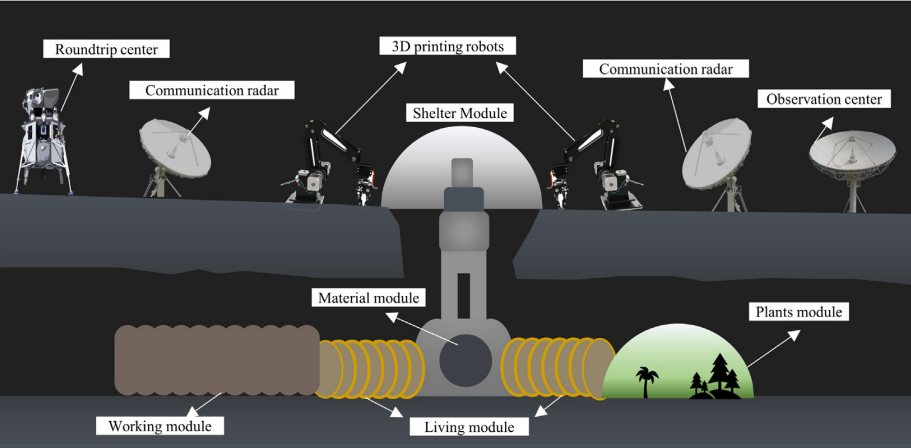
\includegraphics[width=0.8\linewidth]{simple-base-schema.png}
    \caption{Conceptual design of a lunar base within a pit. Overhangs provide natural shielding, while modular inflatable habitats create pressurized living spaces. Adapted from \cite{bases-feng}.}
    \label{fig:lunar-habitat}
\end{figure}

\textbf{Layered Habitat Modules:}
The verticality of lava tubes enables multi-tiered habitat designs, integrating living spaces, laboratories, and storage areas. This approach optimizes spatial utilization while maintaining functionality and safety \cite{sublunear-lava}.

\textbf{Hydroponic Farming Modules:}
The controlled environments within lava tubes are ideal for hydroponic farming, allowing astronauts to cultivate food and sustain life independently of Earth. The lack of surface hazards further supports efficient agricultural operations \cite{bases-feng}.

\subsection{Resource Utilization and Sustainability}

\textbf{Water Extraction:}
Water ice in permanently shadowed regions near pits can be harvested for drinking water, oxygen generation, and fuel production. Technologies such as the extraction of oxygen from regolith complement this effort, enabling closed-loop resource cycles \cite{jsanders-isru}.

\textbf{Energy Solutions:}
Solar panels installed on the surface near pits, combined with tethered power systems, can deliver consistent energy to subsurface habitats. Small modular reactors may complement these systems during lunar nights, ensuring uninterrupted power supply \cite{lro}.

\textbf{Material Processing:}
Using regolith for construction materials through sintering or chemical reduction not only supports structural needs but also enhances mission sustainability by reducing launch payloads \cite{jsanders-isru}.

\subsection{Challenges and Future Directions}

While promising, the habitation of lunar pits and lava tubes presents several challenges:
\begin{itemize}
    \item \textbf{Access and Exploration:} Advanced robotics such as tethered rovers (e.g., Daedalus) and jumping robots are critical for safely exploring and assessing the structural stability of these features \cite{esa-daedalus}.
    \item \textbf{Structural Assessment:} Determining the geological stability of lava tubes and their resistance to collapse is essential for planning long-term habitation \cite{sublunear-lava}.
    \item \textbf{Human Factors:} Prolonged habitation requires addressing psychological and physiological challenges associated with living in isolated, confined environments.
\end{itemize}
